\newpage

\sndEnTeteRevision

\begin{center}
\begin{mdframed}[style=titr, leftmargin=60pt, rightmargin=60pt, innertopmargin=7pt, innerbottommargin=7pt, innerrightmargin=8pt, innerleftmargin=8pt]

\begin{center}
\large{\textbf{Exercices de révisions de collège}}
\end{center}

\end{mdframed}


\end{center}
%Toute l'année, nous utiliserons les outils mathématiques pour décrire des phénomènes physiques et chimiques. Pour être sur d'être bien à l'aise dans l'utilisation de ces outils, voici quelques exercices de révisions, \underline{\textbf{leur résolution ne doit pas vous poser problème}}.\\
Si jamais vous bloquez sur un exercice, n'hésitez pas à revoir vos cours des années précédentes ou, en dernier recours, à me demander en fin de cours pour débloquer la situation.

\renewcommand{\thesubsection}{\textcolor{red}{\textbf{Exercice \arabic{subsection} }}}

\section{Mathématiques}
Tous les exercices suivants doivent être traités \underline{sans calculatrice}.
\subsection{}
\textbf{1.} Effectuer les calculs suivants :
\begin{align*}
    A_1 &= 5 + 3\times20 & A_2 &= \frac{10}{2}\times 8 & A_3 &= \frac{50\times2}{100}-1
\end{align*}
 
 \textbf{2.} Soit $x\in\mathbb{R}$. Développer, réduire et ordonner les expressions suivantes :

 \begin{align*}
B_1 & = 2(x-1)-4(x+5) & B_2 & = 5(3x^2-5)+6(x-2) \\
B_3 & = 3(-1+x)-5(x-7) & B_4 & = 6(x+7)+4x(x-9)  \\
\end{align*}

\subsection{Fractions}
\textbf{1.} Soit $x\in\mathbb{R}$. Réduire les expressions suivantes en une seule fraction irréductible :
\vspace{-0.2cm}
\begin{align*}
A_1 & = \frac{10}{20} & A_2 & = \frac{150}{200} & A_3 &= \frac{9}{81} & A_4 & = \frac{32}{256}
\end{align*}

\textbf{2.} Soit $x\in\mathbb{R}$. Calculer puis exprimer le résultat sous la forme d'une fraction irréductible :

\begin{align*}
    B_1 &= \frac{1}{2}-\frac{1}{3} & B_2 &= \frac{2}{4}+\frac{3}{5} & B_3 &= \frac{19}{38}-\frac{3}{6} & B_4 &= \frac{1}{x}-\frac{x^2}{3x}
\end{align*}

\subsection{Equations du premier degré}
Soit $x$ et $y$ deux inconnues. Résoudre les équations suivantes :
\begin{align*}
    2x &= 10 & 5x+2 &= 8 & 3y + 5x &= 5x + 8 \\
    5y + 2y - 49 &= 0 & \frac{2y^3-5y^2}{y^2} &= 8+y & 
\end{align*}

\subsection{Puissance de 10}
\textit{Exercice très utile pour la physique-chimie !} \\

\textbf{1.} \'{E}crire les nombres suivants sous forme de puissances de 10 :
\vspace{-0.2cm}
\begin{align*}
    A_1 &= 100 & A_2 &= 1 000 000 & A_3 &= 1 & A_4 &= 0, 1 & A_5 &= -10
\end{align*}

\textbf{2.} \'{E}crire les quantités suivantes en notation scientifique :
\vspace{-0.2cm}
\begin{align*}
    B_1 &= 0,15 & B_2 &= 180 & B_3 &= 150 000 009 & B_4 &= 0,00009
\end{align*}

\textbf{3.} Effectuer les calculs suivants :
\vspace{-0.2cm}
\begin{align*}
    C_1 &= 10^{30} \times 10^{50} & C_2 &= \frac{10^{2033}}{10^{10}} & C_3 &= \frac{10^2}{10^8}\times 10^5
\end{align*}

\subsection{Géométrie}
Vous pouvez utiliser la calculatrice pour cet exercice.\textit{Attention, les schémas ne sont pas à l'échelle}.\\

\textbf{1.} En utilisant un théorème de géométrie étudié au collège, montrer que le triangle ci-dessous est rectangle en A :

\begin{figure}[!h]
    \centering
    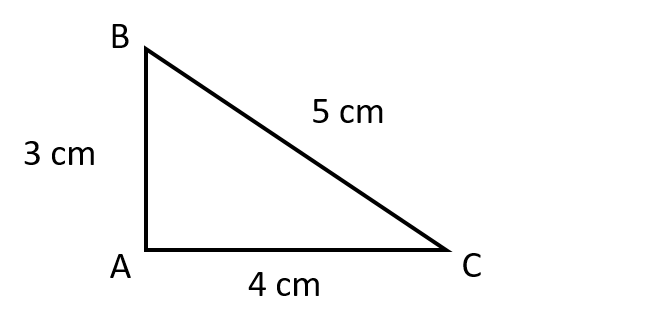
\includegraphics[scale=0.4]{Revision/Triangle_rectangle.png}
\end{figure}
\newpage
\textbf{2.} Le triangle ci-dessous est rectangle en A. Calculer la longueur AC :
\begin{figure}[!h]
    \centering
    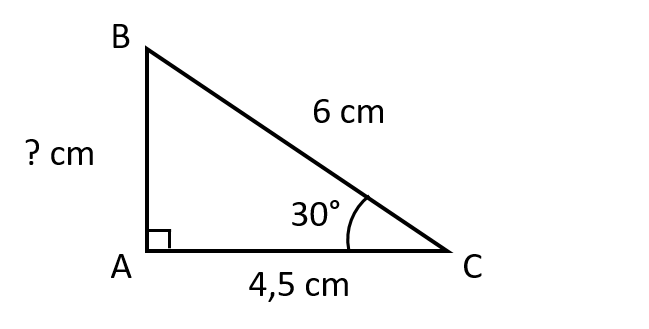
\includegraphics[scale=0.4]{Revision/Triangle_rectangle_2.png}
\end{figure}

\section{Physique}

\subsection{Record de vitesse ferroviaire}
Le projet de train japonais à sustentasion magnétique, le SCMaglev, a atteint la vitesse record de $603$~km/h en 2015. Ce train a la particularité de léviter au-dessus des rails. Pour rappel, un TGV roule à une vitesse de l'ordre de $300$~km/h en France.\\
\begin{enumerate}
    \item Convertir les deux vitesses en $m/s$.
    \item La distance entre Paris et Brest est de 500 km. En combien de temps une voiture roulant en moyenne à $100$~km/h effectue-t-elle ce trajet ? Et un TGV ? Et un SCMaglev ?
    \item Sachant que la distance Terre-Lune est de $380 000$~km, en combien de temps un SCMaglev peut-il atteindre la Lune ? On donnera la réponse en années/ jours/heures/minutes/secondes.
    \item A votre avis, quels sont les avantages du SCMaglev ?
\end{enumerate}

\subsection{Electricité}
\begin{enumerate}
    \item Avec quel instrument mesure-t-on une tension ? En quelle unité exprime-t-on le résultat ?
    \item Mêmes questions pour un courant.
    \item Une ampoule électrique est traversée par un courant I = $0,5$~A, et la tension à ses bornes est $U= 6$~V. Quelle est sa résistance ? Quelle puissance électrique $P$ consomme-t-elle ? 
    \item Faut-il utiliser un fil de cuivre ou un fil en caoutchouc pour conduire le courant ?
\end{enumerate}

\subsection{\'{E}nergie}
On rappelle qu’un corps de masse $m$ se déplaçant à la vitesse $v$ possède une énergie cinétique $E_c$ donnée par :
\begin{equation}
    E_c = \frac{1}{2}mv^2
\end{equation}
avec $E_c$ en J (Joule), $v$ en m/s et $m$ en kg.
\begin{enumerate}
    \item Une voiture pèse $m=1,2$ T. Convertir ce résultat en kg.
    \item Si cette voiture roule à $50$~km/h, quelle est son énergie cinétique ?
    \item \textit{(bonus)} On branche pendant $\Delta t =1$~s une centrale nucléaire délivrant $1$~GW de puissance électrique à une voiture de masse $m=1000$~kg. \`{A} quelle vitesse va la voiture au bout de $\Delta t$ si on suppose que toutes l'énergie électrique fournit par la centrale a été convertie en énergie cinétique ?
\end{enumerate}

\section{Chimie}
\subsection{Atomes et petits pois}
\begin{enumerate}
    \item Quelle est la taille approximative d’un atome ? L’exprimer en m sous forme d’une puissance de 10.
    \item Combien d’atomes faut-il aligner pour obtenir une chaîne de longueur 1 mm ?
    \item Quels sont les principaux constituants d’un atome ?
    \item Modéliser physiquement un petit pois (forme, taille, ...). Si le noyau d’un atome avait la taille d’un petit pois, quelle taille aurait l’atome entier ?
\end{enumerate} 

\subsection{Verrerie}
\textbf{1.} Nommer la verrerie présentée ci-dessous :
\begin{figure}[!h]
    \centering
    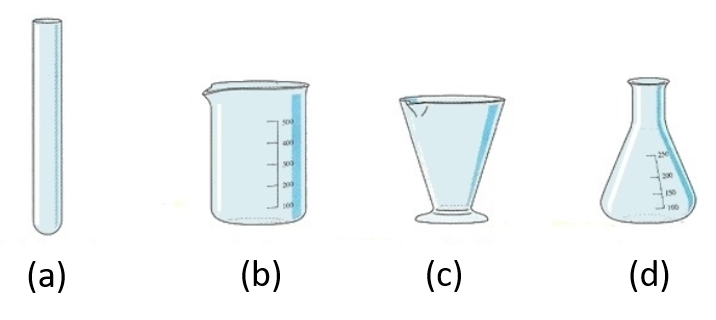
\includegraphics[scale=0.4]{Revision/Verrerie1.png}
\end{figure}

\textbf{2.} Proposer deux méthodes pour peser une masse $m=10$~g d'eau. On rappelle que la masse volumique de l'eau vaut $\rho=1$~g.mL${-1}$.